% Options for packages loaded elsewhere
\PassOptionsToPackage{unicode}{hyperref}
\PassOptionsToPackage{hyphens}{url}
%
\documentclass[
  10pt,
  ignorenonframetext,
  serif]{beamer}
\usepackage{pgfpages}
\setbeamertemplate{caption}[numbered]
\setbeamertemplate{caption label separator}{: }
\setbeamercolor{caption name}{fg=normal text.fg}
\beamertemplatenavigationsymbolsempty
% Prevent slide breaks in the middle of a paragraph
\widowpenalties 1 10000
\raggedbottom
\setbeamertemplate{part page}{
  \centering
  \begin{beamercolorbox}[sep=16pt,center]{part title}
    \usebeamerfont{part title}\insertpart\par
  \end{beamercolorbox}
}
\setbeamertemplate{section page}{
  \centering
  \begin{beamercolorbox}[sep=12pt,center]{part title}
    \usebeamerfont{section title}\insertsection\par
  \end{beamercolorbox}
}
\setbeamertemplate{subsection page}{
  \centering
  \begin{beamercolorbox}[sep=8pt,center]{part title}
    \usebeamerfont{subsection title}\insertsubsection\par
  \end{beamercolorbox}
}
\AtBeginPart{
  \frame{\partpage}
}
\AtBeginSection{
  \ifbibliography
  \else
    \frame{\sectionpage}
  \fi
}
\AtBeginSubsection{
  \frame{\subsectionpage}
}
\usepackage{lmodern}
\usepackage{amssymb,amsmath}
\usepackage{ifxetex,ifluatex}
\ifnum 0\ifxetex 1\fi\ifluatex 1\fi=0 % if pdftex
  \usepackage[T1]{fontenc}
  \usepackage[utf8]{inputenc}
  \usepackage{textcomp} % provide euro and other symbols
\else % if luatex or xetex
  \usepackage{unicode-math}
  \defaultfontfeatures{Scale=MatchLowercase}
  \defaultfontfeatures[\rmfamily]{Ligatures=TeX,Scale=1}
\fi
\usetheme[]{Boadilla}
% Use upquote if available, for straight quotes in verbatim environments
\IfFileExists{upquote.sty}{\usepackage{upquote}}{}
\IfFileExists{microtype.sty}{% use microtype if available
  \usepackage[]{microtype}
  \UseMicrotypeSet[protrusion]{basicmath} % disable protrusion for tt fonts
}{}
\makeatletter
\@ifundefined{KOMAClassName}{% if non-KOMA class
  \IfFileExists{parskip.sty}{%
    \usepackage{parskip}
  }{% else
    \setlength{\parindent}{0pt}
    \setlength{\parskip}{6pt plus 2pt minus 1pt}}
}{% if KOMA class
  \KOMAoptions{parskip=half}}
\makeatother
\usepackage{xcolor}
\IfFileExists{xurl.sty}{\usepackage{xurl}}{} % add URL line breaks if available
\IfFileExists{bookmark.sty}{\usepackage{bookmark}}{\usepackage{hyperref}}
\hypersetup{
  pdftitle={FE8828 Programming Web Applications in Finance},
  pdfauthor={Dr.~Yang Ye ~yy@runchee.com},
  hidelinks,
  pdfcreator={LaTeX via pandoc}}
\urlstyle{same} % disable monospaced font for URLs
\newif\ifbibliography
\usepackage{color}
\usepackage{fancyvrb}
\newcommand{\VerbBar}{|}
\newcommand{\VERB}{\Verb[commandchars=\\\{\}]}
\DefineVerbatimEnvironment{Highlighting}{Verbatim}{commandchars=\\\{\}}
% Add ',fontsize=\small' for more characters per line
\usepackage{framed}
\definecolor{shadecolor}{RGB}{248,248,248}
\newenvironment{Shaded}{\begin{snugshade}}{\end{snugshade}}
\newcommand{\AlertTok}[1]{\textcolor[rgb]{0.94,0.16,0.16}{#1}}
\newcommand{\AnnotationTok}[1]{\textcolor[rgb]{0.56,0.35,0.01}{\textbf{\textit{#1}}}}
\newcommand{\AttributeTok}[1]{\textcolor[rgb]{0.77,0.63,0.00}{#1}}
\newcommand{\BaseNTok}[1]{\textcolor[rgb]{0.00,0.00,0.81}{#1}}
\newcommand{\BuiltInTok}[1]{#1}
\newcommand{\CharTok}[1]{\textcolor[rgb]{0.31,0.60,0.02}{#1}}
\newcommand{\CommentTok}[1]{\textcolor[rgb]{0.56,0.35,0.01}{\textit{#1}}}
\newcommand{\CommentVarTok}[1]{\textcolor[rgb]{0.56,0.35,0.01}{\textbf{\textit{#1}}}}
\newcommand{\ConstantTok}[1]{\textcolor[rgb]{0.00,0.00,0.00}{#1}}
\newcommand{\ControlFlowTok}[1]{\textcolor[rgb]{0.13,0.29,0.53}{\textbf{#1}}}
\newcommand{\DataTypeTok}[1]{\textcolor[rgb]{0.13,0.29,0.53}{#1}}
\newcommand{\DecValTok}[1]{\textcolor[rgb]{0.00,0.00,0.81}{#1}}
\newcommand{\DocumentationTok}[1]{\textcolor[rgb]{0.56,0.35,0.01}{\textbf{\textit{#1}}}}
\newcommand{\ErrorTok}[1]{\textcolor[rgb]{0.64,0.00,0.00}{\textbf{#1}}}
\newcommand{\ExtensionTok}[1]{#1}
\newcommand{\FloatTok}[1]{\textcolor[rgb]{0.00,0.00,0.81}{#1}}
\newcommand{\FunctionTok}[1]{\textcolor[rgb]{0.00,0.00,0.00}{#1}}
\newcommand{\ImportTok}[1]{#1}
\newcommand{\InformationTok}[1]{\textcolor[rgb]{0.56,0.35,0.01}{\textbf{\textit{#1}}}}
\newcommand{\KeywordTok}[1]{\textcolor[rgb]{0.13,0.29,0.53}{\textbf{#1}}}
\newcommand{\NormalTok}[1]{#1}
\newcommand{\OperatorTok}[1]{\textcolor[rgb]{0.81,0.36,0.00}{\textbf{#1}}}
\newcommand{\OtherTok}[1]{\textcolor[rgb]{0.56,0.35,0.01}{#1}}
\newcommand{\PreprocessorTok}[1]{\textcolor[rgb]{0.56,0.35,0.01}{\textit{#1}}}
\newcommand{\RegionMarkerTok}[1]{#1}
\newcommand{\SpecialCharTok}[1]{\textcolor[rgb]{0.00,0.00,0.00}{#1}}
\newcommand{\SpecialStringTok}[1]{\textcolor[rgb]{0.31,0.60,0.02}{#1}}
\newcommand{\StringTok}[1]{\textcolor[rgb]{0.31,0.60,0.02}{#1}}
\newcommand{\VariableTok}[1]{\textcolor[rgb]{0.00,0.00,0.00}{#1}}
\newcommand{\VerbatimStringTok}[1]{\textcolor[rgb]{0.31,0.60,0.02}{#1}}
\newcommand{\WarningTok}[1]{\textcolor[rgb]{0.56,0.35,0.01}{\textbf{\textit{#1}}}}
\setlength{\emergencystretch}{3em} % prevent overfull lines
\providecommand{\tightlist}{%
  \setlength{\itemsep}{0pt}\setlength{\parskip}{0pt}}
\setcounter{secnumdepth}{-\maxdimen} % remove section numbering
\usepackage{fourier}
\ifluatex
  \usepackage{selnolig}  % disable illegal ligatures
\fi

\title{FE8828 Programming Web Applications in Finance}
\subtitle{Week 2: 1. R Programming/2 2. R Shiny/2: Building a web app 3.
dplyr/1: Data Manipulation}
\author{Dr.~Yang Ye
~\href{mailto:yy@runchee.com}{\nolinkurl{yy@runchee.com}}}
\date{Sep 24, 2020}
\institute{Nanyang Business School}

\begin{document}
\frame{\titlepage}

\begin{frame}[allowframebreaks]
  \tableofcontents[hideallsubsections]
\end{frame}
\begin{frame}
\end{frame}

\begin{frame}[fragile]{Object}
\protect\hypertarget{object}{}
S3 Object System in R

\begin{Shaded}
\begin{Highlighting}[]
\CommentTok{\# Object}
\CommentTok{\# Define class with attributes.}
\NormalTok{vanilla\_option \textless{}{-}}\StringTok{ }\KeywordTok{setClass}\NormalTok{(}\StringTok{"vanilla\_option"}\NormalTok{,}
                           \DataTypeTok{slots =} \KeywordTok{c}\NormalTok{(}\DataTypeTok{type =} \StringTok{"character"}\NormalTok{,}
                                     \DataTypeTok{strike =} \StringTok{"numeric"}\NormalTok{,}
                                     \DataTypeTok{underlying =} \StringTok{"numeric"}\NormalTok{))}

\CommentTok{\# Create object, either way}
\NormalTok{opt1 \textless{}{-}}\StringTok{ }\KeywordTok{new}\NormalTok{(}\StringTok{"vanilla\_option"}\NormalTok{, }\DataTypeTok{type =} \StringTok{"c"}\NormalTok{, }\DataTypeTok{strike =} \DecValTok{100}\NormalTok{, }\DataTypeTok{underlying =} \DecValTok{100}\NormalTok{)}
\NormalTok{opt2 \textless{}{-}}\StringTok{ }\KeywordTok{vanilla\_option}\NormalTok{(}\DataTypeTok{type =} \StringTok{"c"}\NormalTok{, }\DataTypeTok{strike =} \DecValTok{100}\NormalTok{, }\DataTypeTok{underlying =} \DecValTok{100}\NormalTok{)}

\CommentTok{\# Use @ to visit member. or,}
\NormalTok{opt1}\OperatorTok{@}\NormalTok{type}
\CommentTok{\#\# [1] "c"}
\KeywordTok{slot}\NormalTok{(opt1, }\StringTok{"strike"}\NormalTok{)}
\CommentTok{\#\# [1] 100}
\end{Highlighting}
\end{Shaded}
\end{frame}

\begin{frame}[fragile]{Work with objects}
\protect\hypertarget{work-with-objects}{}
\begin{Shaded}
\begin{Highlighting}[]
\CommentTok{\# Generate a vector of options}
\NormalTok{opts \textless{}{-}}\StringTok{ }\KeywordTok{sapply}\NormalTok{(}\DecValTok{1}\OperatorTok{:}\DecValTok{10000}\NormalTok{, }\ControlFlowTok{function}\NormalTok{(x) \{ }
                          \KeywordTok{vanilla\_option}\NormalTok{(}\DataTypeTok{type =} \KeywordTok{sample}\NormalTok{(}\KeywordTok{c}\NormalTok{(}\StringTok{"c"}\NormalTok{, }\StringTok{"p"}\NormalTok{), }\DecValTok{1}\NormalTok{),}
                                         \DataTypeTok{strike =} \KeywordTok{round}\NormalTok{(}\KeywordTok{runif}\NormalTok{(}\DecValTok{1}\NormalTok{) }\OperatorTok{*}\StringTok{ }\DecValTok{100}\NormalTok{, }\DecValTok{0}\NormalTok{),}
                                         \DataTypeTok{underlying =} \KeywordTok{round}\NormalTok{(}\KeywordTok{runif}\NormalTok{(}\DecValTok{1}\NormalTok{) }\OperatorTok{*}\StringTok{ }\DecValTok{100}\NormalTok{, }\DecValTok{0}\NormalTok{)) \})}

\CommentTok{\# install.packages("fOptions")}
\KeywordTok{library}\NormalTok{(fOptions)}

\NormalTok{start \textless{}{-}}\StringTok{ }\KeywordTok{Sys.time}\NormalTok{()}
\CommentTok{\# GBSOption also returns an object. We just need its price attribute.}
\NormalTok{res1 \textless{}{-}}\StringTok{ }\KeywordTok{sapply}\NormalTok{(opts, }\ControlFlowTok{function}\NormalTok{(o) \{}
\NormalTok{  obj \textless{}{-}}\StringTok{ }\KeywordTok{GBSOption}\NormalTok{(o}\OperatorTok{@}\NormalTok{type, o}\OperatorTok{@}\NormalTok{underlying, o}\OperatorTok{@}\NormalTok{strike, }\DataTypeTok{Time =} \DecValTok{1}\NormalTok{,}
             \DataTypeTok{r =} \FloatTok{0.01}\NormalTok{, }\DataTypeTok{b =} \DecValTok{0}\NormalTok{, }\DataTypeTok{sigma =} \FloatTok{0.3}\NormalTok{)}
\NormalTok{  obj}\OperatorTok{@}\NormalTok{price}
\NormalTok{\})}
\KeywordTok{cat}\NormalTok{(}\KeywordTok{as.numeric}\NormalTok{(}\KeywordTok{Sys.time}\NormalTok{() }\OperatorTok{{-}}\StringTok{ }\NormalTok{start))}
\CommentTok{\#\# 14.50904}
\KeywordTok{head}\NormalTok{(res1, }\DataTypeTok{n =} \DecValTok{4}\NormalTok{)}
\CommentTok{\#\# [1]  0.3837668  5.7844016  0.0000000 31.8493122}

\CommentTok{\# Alternatively to sapply, we can use map* functions from purrr package}
\CommentTok{\# map is a generic function that returns a list}
\CommentTok{\# map\_dbl is for result of double, it would return a vector}
\KeywordTok{library}\NormalTok{(purrr)}

\NormalTok{res2 \textless{}{-}}\StringTok{ }\NormalTok{purrr}\OperatorTok{::}\KeywordTok{map\_dbl}\NormalTok{(opts, }\ControlFlowTok{function}\NormalTok{(o) \{}
\NormalTok{  (}\KeywordTok{GBSOption}\NormalTok{(o}\OperatorTok{@}\NormalTok{type, o}\OperatorTok{@}\NormalTok{underlying, o}\OperatorTok{@}\NormalTok{strike, }\DataTypeTok{Time =} \DecValTok{1}\NormalTok{,}
             \DataTypeTok{r =} \FloatTok{0.01}\NormalTok{, }\DataTypeTok{b =} \DecValTok{0}\NormalTok{, }\DataTypeTok{sigma =} \FloatTok{0.3}\NormalTok{))}\OperatorTok{@}\NormalTok{price}
\NormalTok{\})}
\KeywordTok{head}\NormalTok{(res2, }\DataTypeTok{n =} \DecValTok{4}\NormalTok{)}
\CommentTok{\#\# [1]  0.3837668  5.7844016  0.0000000 31.8493122}
\end{Highlighting}
\end{Shaded}
\end{frame}

\begin{frame}[fragile]{Read/Write data}
\protect\hypertarget{readwrite-data}{}
\begin{Shaded}
\begin{Highlighting}[]
\CommentTok{\# set working directory}
\KeywordTok{setwd}\NormalTok{(}\StringTok{"C:/TEMP"}\NormalTok{)}
\CommentTok{\# Save this\_is\_var1 to a file}
\KeywordTok{saveRDS}\NormalTok{(this\_is\_var1, }\DataTypeTok{file =} \StringTok{"C:/TEMP/DATA/data.Rds"}\NormalTok{)}
\CommentTok{\# Load a variable from a file. \textasciigrave{}new\_loaded\textasciigrave{} is the name given to it.}
\NormalTok{new\_loaded \textless{}{-}}\StringTok{ }\KeywordTok{readRDS}\NormalTok{(}\DataTypeTok{file =} \StringTok{"C:/TEMP/DATA/data.Rds"}\NormalTok{)}
\end{Highlighting}
\end{Shaded}

\begin{itemize}
\tightlist
\item
  On Windows, use double slashes
  \texttt{\textbackslash{}\textbackslash{}} or single backslash
  \texttt{/}.
  e.g.~\texttt{C:\textbackslash{}\textbackslash{}TEMP\textbackslash{}\textbackslash{}DATA},
  \texttt{C:/TEMP/DATA}
\item
  On Mac, use backslash \texttt{/Users/.../}
\end{itemize}
\end{frame}

\begin{frame}[fragile]{Exercise 1: Fastest Fish Problem}
\protect\hypertarget{exercise-1-fastest-fish-problem}{}
We have ten fishes releases in a very long lane at fixed time interval.
They swim at different speed. The fish surpassing the previous fish
would eat it. How many fishes would survive on average?

\begin{verbatim}
## Warning in text.default(res$queue[i], i, paste0("<U+2653> ", i), col =
## "skyblue3", : conversion failure on '♓ 1' in 'mbcsToSbcs': dot substituted for
## <e2>
## Warning in text.default(res$queue[i], i, paste0("<U+2653> ", i), col =
## "skyblue3", : conversion failure on '♓ 1' in 'mbcsToSbcs': dot substituted for
## <99>
## Warning in text.default(res$queue[i], i, paste0("<U+2653> ", i), col =
## "skyblue3", : conversion failure on '♓ 1' in 'mbcsToSbcs': dot substituted for
## <93>
## Warning in text.default(res$queue[i], i, paste0("<U+2653> ", i), col =
## "skyblue3", : font metrics unknown for Unicode character U+2653
## Warning in text.default(res$queue[i], i, paste0("<U+2653> ", i), col =
## "skyblue3", : conversion failure on '♓ 2' in 'mbcsToSbcs': dot substituted for
## <e2>
## Warning in text.default(res$queue[i], i, paste0("<U+2653> ", i), col =
## "skyblue3", : conversion failure on '♓ 2' in 'mbcsToSbcs': dot substituted for
## <99>
## Warning in text.default(res$queue[i], i, paste0("<U+2653> ", i), col =
## "skyblue3", : conversion failure on '♓ 2' in 'mbcsToSbcs': dot substituted for
## <93>
## Warning in text.default(res$queue[i], i, paste0("<U+2653> ", i), col =
## "skyblue3", : font metrics unknown for Unicode character U+2653
## Warning in text.default(res$queue[i], i, paste0("<U+2653> ", i), col =
## "skyblue3", : conversion failure on '♓ 3' in 'mbcsToSbcs': dot substituted for
## <e2>
## Warning in text.default(res$queue[i], i, paste0("<U+2653> ", i), col =
## "skyblue3", : conversion failure on '♓ 3' in 'mbcsToSbcs': dot substituted for
## <99>
## Warning in text.default(res$queue[i], i, paste0("<U+2653> ", i), col =
## "skyblue3", : conversion failure on '♓ 3' in 'mbcsToSbcs': dot substituted for
## <93>
## Warning in text.default(res$queue[i], i, paste0("<U+2653> ", i), col =
## "skyblue3", : font metrics unknown for Unicode character U+2653
## Warning in text.default(res$qori[i], i, paste0("<U+2653> ", i), col = "grey", :
## conversion failure on '♓ 4' in 'mbcsToSbcs': dot substituted for <e2>
## Warning in text.default(res$qori[i], i, paste0("<U+2653> ", i), col = "grey", :
## conversion failure on '♓ 4' in 'mbcsToSbcs': dot substituted for <99>
## Warning in text.default(res$qori[i], i, paste0("<U+2653> ", i), col = "grey", :
## conversion failure on '♓ 4' in 'mbcsToSbcs': dot substituted for <93>
## Warning in text.default(res$qori[i], i, paste0("<U+2653> ", i), col = "grey", :
## font metrics unknown for Unicode character U+2653
## Warning in text.default(res$queue[i], i, paste0("<U+2653> ", i), col =
## "skyblue3", : conversion failure on '♓ 5' in 'mbcsToSbcs': dot substituted for
## <e2>
## Warning in text.default(res$queue[i], i, paste0("<U+2653> ", i), col =
## "skyblue3", : conversion failure on '♓ 5' in 'mbcsToSbcs': dot substituted for
## <99>
## Warning in text.default(res$queue[i], i, paste0("<U+2653> ", i), col =
## "skyblue3", : conversion failure on '♓ 5' in 'mbcsToSbcs': dot substituted for
## <93>
## Warning in text.default(res$queue[i], i, paste0("<U+2653> ", i), col =
## "skyblue3", : font metrics unknown for Unicode character U+2653
## Warning in text.default(res$qori[i], i, paste0("<U+2653> ", i), col = "grey", :
## conversion failure on '♓ 6' in 'mbcsToSbcs': dot substituted for <e2>
## Warning in text.default(res$qori[i], i, paste0("<U+2653> ", i), col = "grey", :
## conversion failure on '♓ 6' in 'mbcsToSbcs': dot substituted for <99>
## Warning in text.default(res$qori[i], i, paste0("<U+2653> ", i), col = "grey", :
## conversion failure on '♓ 6' in 'mbcsToSbcs': dot substituted for <93>
## Warning in text.default(res$qori[i], i, paste0("<U+2653> ", i), col = "grey", :
## font metrics unknown for Unicode character U+2653
## Warning in text.default(res$queue[i], i, paste0("<U+2653> ", i), col =
## "skyblue3", : conversion failure on '♓ 7' in 'mbcsToSbcs': dot substituted for
## <e2>
## Warning in text.default(res$queue[i], i, paste0("<U+2653> ", i), col =
## "skyblue3", : conversion failure on '♓ 7' in 'mbcsToSbcs': dot substituted for
## <99>
## Warning in text.default(res$queue[i], i, paste0("<U+2653> ", i), col =
## "skyblue3", : conversion failure on '♓ 7' in 'mbcsToSbcs': dot substituted for
## <93>
## Warning in text.default(res$queue[i], i, paste0("<U+2653> ", i), col =
## "skyblue3", : font metrics unknown for Unicode character U+2653
## Warning in text.default(res$qori[i], i, paste0("<U+2653> ", i), col = "grey", :
## conversion failure on '♓ 8' in 'mbcsToSbcs': dot substituted for <e2>
## Warning in text.default(res$qori[i], i, paste0("<U+2653> ", i), col = "grey", :
## conversion failure on '♓ 8' in 'mbcsToSbcs': dot substituted for <99>
## Warning in text.default(res$qori[i], i, paste0("<U+2653> ", i), col = "grey", :
## conversion failure on '♓ 8' in 'mbcsToSbcs': dot substituted for <93>
## Warning in text.default(res$qori[i], i, paste0("<U+2653> ", i), col = "grey", :
## font metrics unknown for Unicode character U+2653
## Warning in text.default(res$qori[i], i, paste0("<U+2653> ", i), col = "grey", :
## conversion failure on '♓ 9' in 'mbcsToSbcs': dot substituted for <e2>
## Warning in text.default(res$qori[i], i, paste0("<U+2653> ", i), col = "grey", :
## conversion failure on '♓ 9' in 'mbcsToSbcs': dot substituted for <99>
## Warning in text.default(res$qori[i], i, paste0("<U+2653> ", i), col = "grey", :
## conversion failure on '♓ 9' in 'mbcsToSbcs': dot substituted for <93>
## Warning in text.default(res$qori[i], i, paste0("<U+2653> ", i), col = "grey", :
## font metrics unknown for Unicode character U+2653
## Warning in text.default(res$qori[i], i, paste0("<U+2653> ", i), col = "grey", :
## conversion failure on '♓ 10' in 'mbcsToSbcs': dot substituted for <e2>
## Warning in text.default(res$qori[i], i, paste0("<U+2653> ", i), col = "grey", :
## conversion failure on '♓ 10' in 'mbcsToSbcs': dot substituted for <99>
## Warning in text.default(res$qori[i], i, paste0("<U+2653> ", i), col = "grey", :
## conversion failure on '♓ 10' in 'mbcsToSbcs': dot substituted for <93>
## Warning in text.default(res$qori[i], i, paste0("<U+2653> ", i), col = "grey", :
## font metrics unknown for Unicode character U+2653
\end{verbatim}

\begin{center}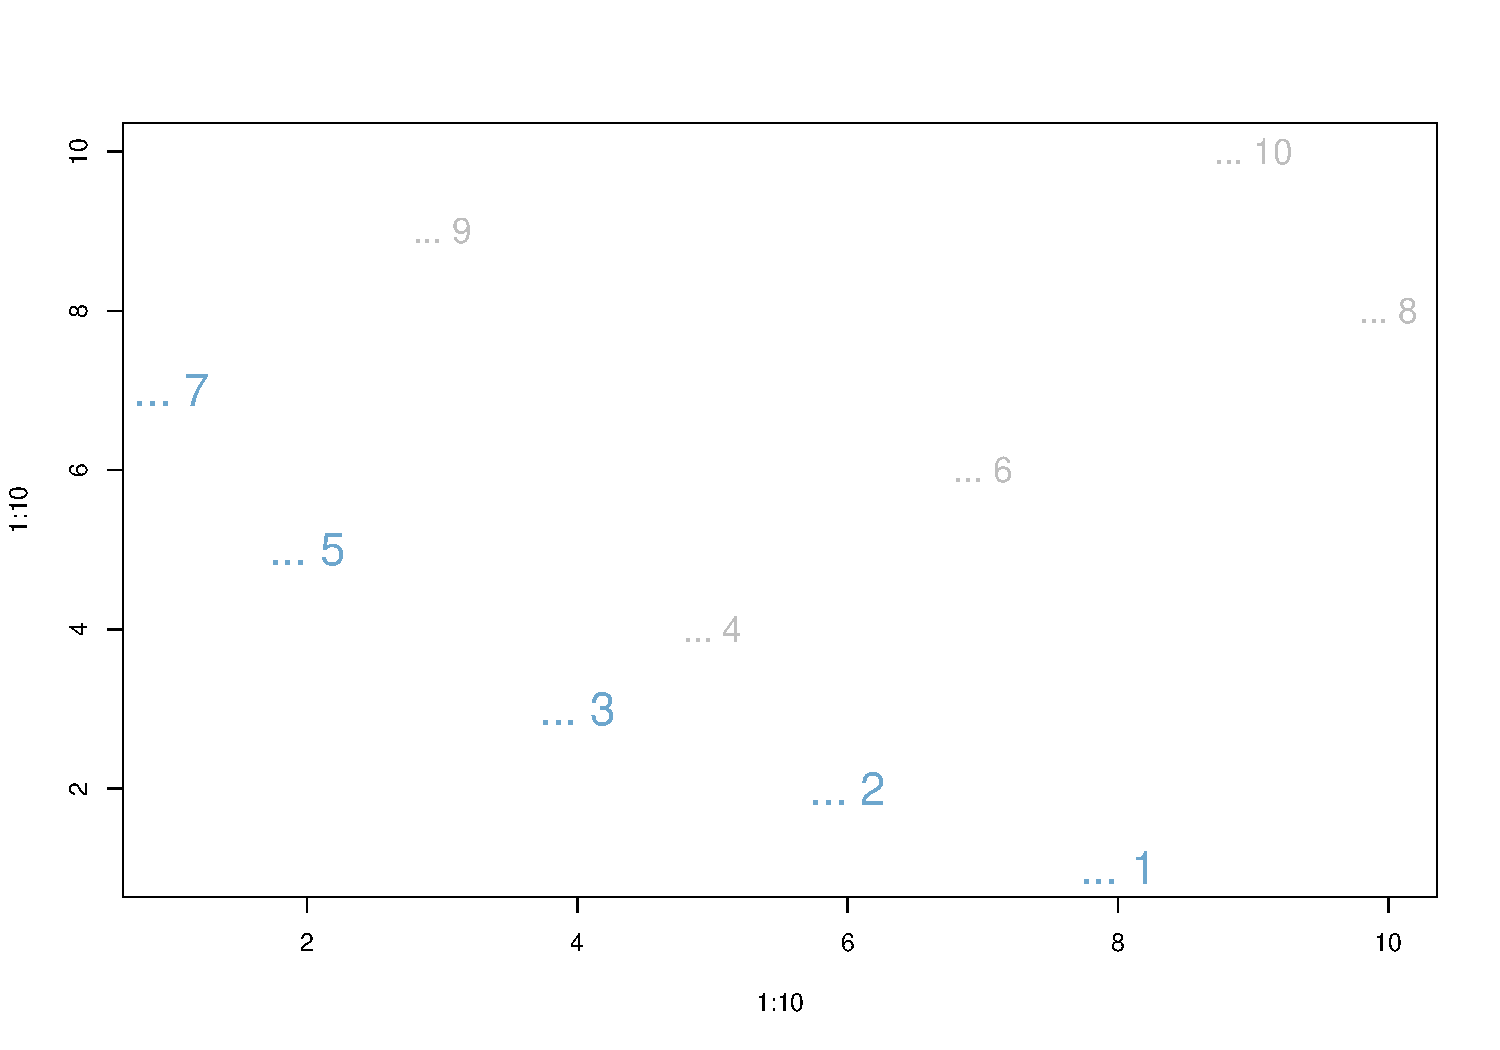
\includegraphics{lec04_files/figure-beamer/unnamed-chunk-4-1} \end{center}
\end{frame}

\begin{frame}[fragile]{Histogram of Fishes Alive}
\protect\hypertarget{histogram-of-fishes-alive}{}
\begin{verbatim}
## res_sim: 2.9425
## res_ana: 2.92896825396825
\end{verbatim}

\begin{center}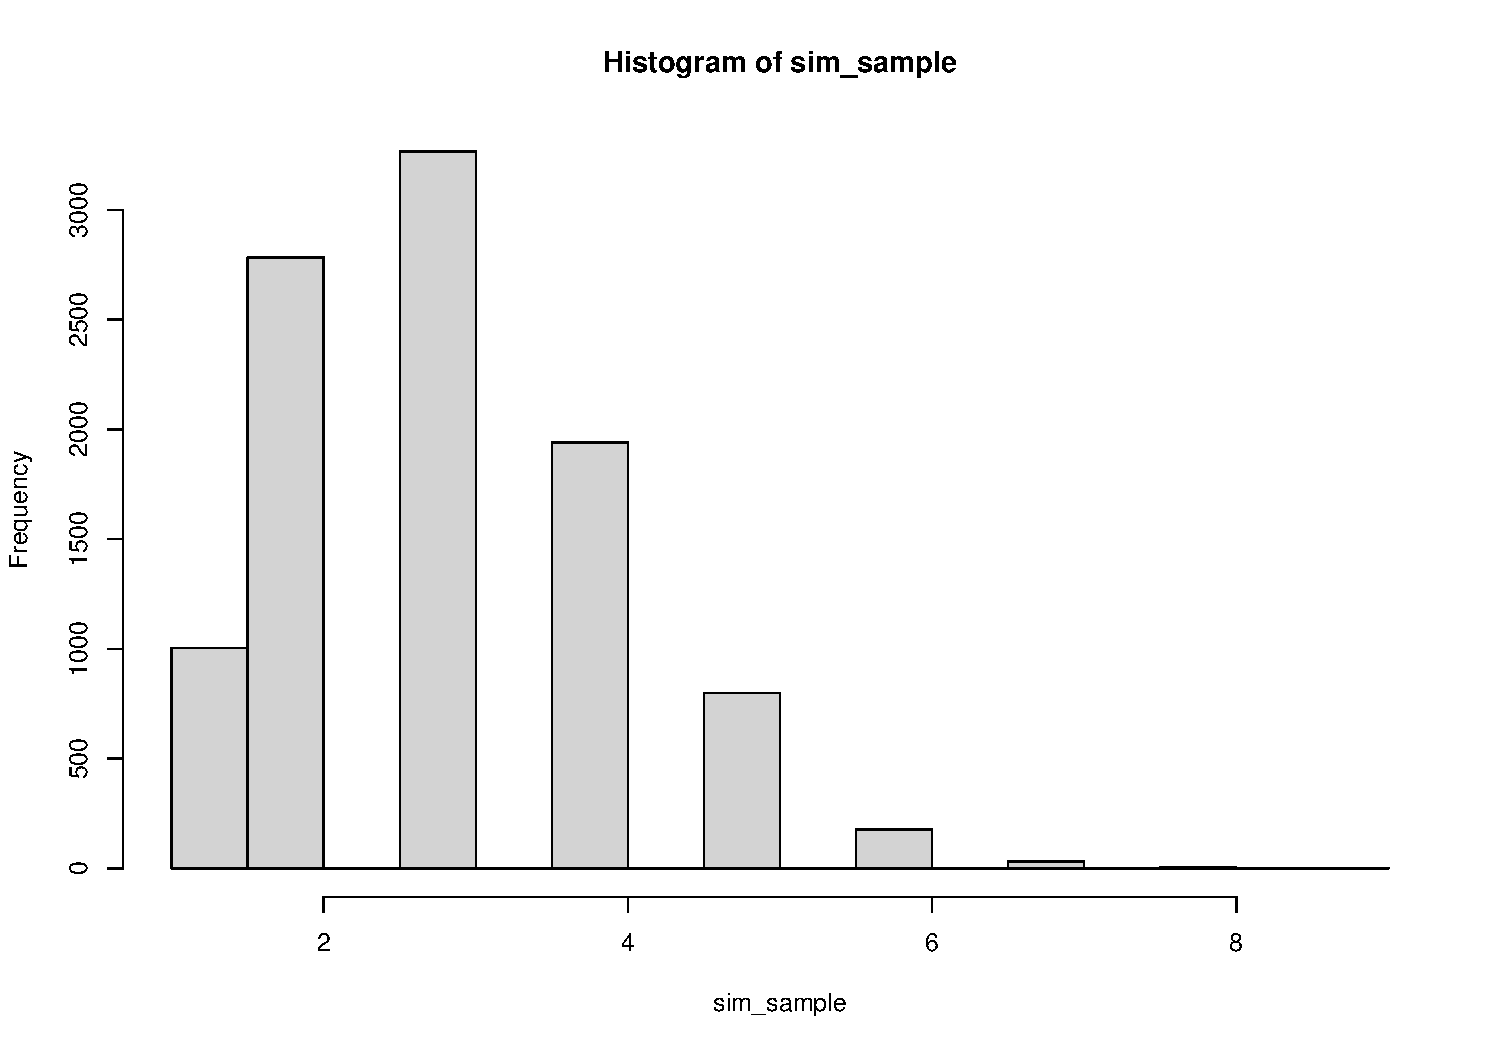
\includegraphics{lec04_files/figure-beamer/unnamed-chunk-5-1} \end{center}
\end{frame}

\begin{frame}[fragile]{Exercise 2: How far to make a choice?}
\protect\hypertarget{exercise-2-how-far-to-make-a-choice}{}
\begin{itemize}
\tightlist
\item
  Secretary Problem
  (\url{https://en.wikipedia.org/wiki/Secretary_problem})
\item
  If we have 100 secretaries ranked from best to worst, coming to
  interview at random order, what's the probability that our picked is
  the best in the group?
\item
  Our selection strategy, use a small group to establish our selection
  criteria, for the subsequent ones, we pick the first that's better
  than our selection criteria. What's the split?
\end{itemize}

Step 1: make\_choice \textless- function(N, split\_number)

\begin{enumerate}
\tightlist
\item
  Generate a list \texttt{input\_list} of \texttt{N} long with integer 1
  to N at random position
\item
  Split the list \texttt{input\_list} into two: evaluation group and
  selection group.
\item
  Remember the best number from evaluaton group and match the first
  number in selection group, \textgreater= than best. Return it.
\end{enumerate}

Run this function for a few (hundred) times and find the probability of
getting N.

Step 2: find\_optimal(), calls Step 1 a few (hundred) times for each of
the split number from 1 to N/2. So we can find the optimal value for the
split for the N.

Hint: Find the solution for N = 3, and N = 10, then move on to N = 100.
\end{frame}

\hypertarget{lecture-5-shiny2-r-web-framework}{%
\section{Lecture 5: Shiny/2: R Web
Framework}\label{lecture-5-shiny2-r-web-framework}}

\begin{frame}[fragile]{Minimalist}
\protect\hypertarget{minimalist}{}
\begin{Shaded}
\begin{Highlighting}[]
\KeywordTok{library}\NormalTok{(shiny)}
\NormalTok{ui \textless{}{-}}\StringTok{ }\KeywordTok{fluidPage}\NormalTok{(}\StringTok{"Hello World"}\NormalTok{)}
\NormalTok{server \textless{}{-}}\StringTok{ }\ControlFlowTok{function}\NormalTok{(input, output, session) \{ \}}
\KeywordTok{shinyApp}\NormalTok{(}\DataTypeTok{ui =}\NormalTok{ ui, }\DataTypeTok{server =}\NormalTok{ server)}
\end{Highlighting}
\end{Shaded}
\end{frame}

\begin{frame}[fragile]{Think around Input and Outputs}
\protect\hypertarget{think-around-input-and-outputs}{}
\begin{Shaded}
\begin{Highlighting}[]
\NormalTok{ui \textless{}{-}}\StringTok{ }\KeywordTok{fluidPage}\NormalTok{(}
  \KeywordTok{titlePanel}\NormalTok{(}\StringTok{"Hello World with a Histogram"}\NormalTok{),}
  \CommentTok{\# Input() functions}
  \KeywordTok{numericInput}\NormalTok{(}\StringTok{"num"}\NormalTok{, }\StringTok{"Number of Sample"}\NormalTok{, }\DataTypeTok{value =} \DecValTok{30}\NormalTok{),}
  \CommentTok{\# Output() functions}
  \KeywordTok{plotOutput}\NormalTok{(}\StringTok{"hist"}\NormalTok{)}
\NormalTok{)}
\end{Highlighting}
\end{Shaded}
\end{frame}

\begin{frame}[fragile]{Input}
\protect\hypertarget{input}{}
All input function follow such function signature except for
input-specific parameters.

\begin{Shaded}
\begin{Highlighting}[]
\KeywordTok{inputXXX}\NormalTok{(}\DataTypeTok{inputId =} \StringTok{"input name"}\NormalTok{, }\DataTypeTok{label =} \StringTok{"label to display"}\NormalTok{, ...)}
\end{Highlighting}
\end{Shaded}

\begin{itemize}
\tightlist
\item
  \texttt{numericInput}
\item
  \texttt{textInput}
\item
  \texttt{passwordInput}
\item
  \texttt{slideInput}
\item
  \texttt{selectInput}
\item
  \texttt{dateInput}
\end{itemize}

Reference: \url{https://shiny.rstudio.com/reference/shiny/1.1.0/}
\end{frame}

\begin{frame}[fragile]{Output}
\protect\hypertarget{output}{}
All output functions follow such pattern.

\begin{Shaded}
\begin{Highlighting}[]
\KeywordTok{yyyOutput}\NormalTok{(}\DataTypeTok{outputId =} \StringTok{"output name"}\NormalTok{)}
\end{Highlighting}
\end{Shaded}

\begin{itemize}
\tightlist
\item
  \texttt{textOutput("text")}
\item
  \texttt{verbatimTextOutput("text\_orignal")}
\item
  \texttt{tableOutput("t1")}
\item
  \texttt{dataTableOutput("t2")}
\item
  \texttt{plotOutput(outputId\ =\ "hist",\ width\ =\ "400px",\ height\ =\ "400px")}
\item
  \texttt{uiOutput("uiX")}
\end{itemize}

For plotOutput, I suggest to set width and height to fixed size so we
need extra parameters. For other kinds of outputs, only
\texttt{outputId} is good enough.
\end{frame}

\begin{frame}[fragile]{Server}
\protect\hypertarget{server}{}
Sever is to fill the content of output

\begin{Shaded}
\begin{Highlighting}[]
\NormalTok{server \textless{}{-}}\StringTok{ }\ControlFlowTok{function}\NormalTok{(input, output, session) \{}
  \CommentTok{\# Enable either one of two}
\NormalTok{  output}\OperatorTok{$}\NormalTok{hist \textless{}{-}}\StringTok{ }\KeywordTok{renderPlot}\NormalTok{(\{ }\KeywordTok{hist}\NormalTok{(}\KeywordTok{rnorm}\NormalTok{(}\DecValTok{100}\NormalTok{)) \})}
  
  \ControlFlowTok{if}\NormalTok{ (}\OtherTok{FALSE}\NormalTok{) \{}
\NormalTok{    output}\OperatorTok{$}\NormalTok{hist \textless{}{-}}\StringTok{ }\KeywordTok{renderPlot}\NormalTok{(\{}
      \KeywordTok{title}\NormalTok{(}\StringTok{"a normal random number histogram"}\NormalTok{)}
      \KeywordTok{hist}\NormalTok{(}\KeywordTok{rnorm}\NormalTok{(input}\OperatorTok{$}\NormalTok{num))}
\NormalTok{    \})}
\NormalTok{  \}}
\NormalTok{\}}
\end{Highlighting}
\end{Shaded}
\end{frame}

\begin{frame}[fragile]{shinyApp = UI + Server}
\protect\hypertarget{shinyapp-ui-server}{}
\begin{itemize}
\tightlist
\item
  UI and Server combine to be a ShinyApp.
\item
  UI is to run the same for each browser/client.
\item
  Server is separate between different users.
\end{itemize}

\begin{Shaded}
\begin{Highlighting}[]
\KeywordTok{shinyApp}\NormalTok{(ui, server)}
\end{Highlighting}
\end{Shaded}
\end{frame}

\begin{frame}[fragile]{Reactivity Kicks In}
\protect\hypertarget{reactivity-kicks-in}{}
\begin{itemize}
\tightlist
\item
  Reactivity:
  \texttt{input\$num\ -\/-\/-\/-\/-\/-\textgreater{}\ output\$p1}
\item
  Reactivity links input to the output like a data flow.
\end{itemize}

Reactive values work together with reactive functions.

\begin{enumerate}
\tightlist
\item
  Reactive function responds.
  \texttt{input\$x\ =\textgreater{}\ output\$y}
\item
  Reactive value notifies.
  \texttt{input\$x\ =\textgreater{}\ expression()\ =\textgreater{}\ output\$y}
\end{enumerate}
\end{frame}

\begin{frame}[fragile]{Reactivity - 1}
\protect\hypertarget{reactivity---1}{}
Reactivity is enabled by placing input \texttt{inputXXX} inside
\texttt{renderXXX} function. (shiny-21.R)

\begin{verbatim}
library(shiny)

ui <- fluidPage(
  numericInput("num", "Num", 100),
  # numericInput("mean", "Mean", 5),
  # numericInput("sd", "SD", 3),
  numericInput("lambda", "Lambda", 1),
  plotOutput("p1")
)

server <- function(input, output, session) {
  output$p1 <- renderPlot({
    # hist(rnorm(input$num, mean = input$mean, sd = input$sd))
    hist(rpois(n = input$num, lambda = input$lambda))
  })
}

shinyApp(ui, server)
\end{verbatim}
\end{frame}

\begin{frame}[fragile]{Reactivity - 2}
\protect\hypertarget{reactivity---2}{}
\begin{itemize}
\tightlist
\item
  Button represents a manual trigger of the action.
\item
  We use \texttt{observeEvent} to observe button action, and
  \texttt{isolate} to cut down the link of \texttt{inputXXX} in
  \texttt{renderXXX}, so button can work.
\item
  If we remove \texttt{isolate}? (shiny-22.R)
\end{itemize}

\begin{verbatim}
library(shiny)

ui <- fluidPage(
  numericInput("num", "Num", 10),
  actionButton("go", "Go"),
  plotOutput("p1")
)

server <- function(input, output, session) {
  observeEvent(input$go, {
    output$p1 <- renderPlot({
      # hist(rnorm(isolate(input$num)))
      # To make code in good clarity, I re-write above one line into below two lines
      # with additional variable input_num to hold the value from input$num.
      input_num <- isolate(input$num)
      hist(rnorm(input_num))
    }) 
  })
}

shinyApp(ui, server)
\end{verbatim}
\end{frame}

\begin{frame}[fragile]{Reactivity - 3}
\protect\hypertarget{reactivity---3}{}
We can add a reactiveValue with \texttt{eventReactive}. (shiny-23.R)

\begin{verbatim}
library(shiny)

ui <- fluidPage(
  numericInput("num", "Num", 10),
  actionButton("go", "Go"),
  plotOutput("p1")
)

server <- function(input, output, session) {
  data <- eventReactive(input$go, {
    hist(rnorm(input$num))
  })
  # Variable data becomes a reactive variable.
  # What changes to it will trigger the output.
  output$p1 <- renderPlot({ data() })
}

shinyApp(ui, server)
\end{verbatim}
\end{frame}

\begin{frame}[fragile]{Output}
\protect\hypertarget{output-1}{}
For tableOutput

\begin{Shaded}
\begin{Highlighting}[]
\NormalTok{output}\OperatorTok{$}\NormalTok{t1 \textless{}{-}}\StringTok{ }\KeywordTok{renderTable}\NormalTok{(iris)}

\NormalTok{output}\OperatorTok{$}\NormalTok{t1 \textless{}{-}}\StringTok{ }\KeywordTok{renderTable}\NormalTok{(\{}
\NormalTok{  some input..}
\NormalTok{  output is a data frame.}
\NormalTok{\})}
\end{Highlighting}
\end{Shaded}

For dataTableOutput (Dynamic table)

\begin{Shaded}
\begin{Highlighting}[]
\NormalTok{output}\OperatorTok{$}\NormalTok{t2 \textless{}{-}}\StringTok{ }\KeywordTok{renderDataTable}\NormalTok{(iris)}
\end{Highlighting}
\end{Shaded}

For plotOutput

\begin{Shaded}
\begin{Highlighting}[]
\NormalTok{output}\OperatorTok{$}\NormalTok{p2 \textless{}{-}}\StringTok{ }\KeywordTok{renderPlot}\NormalTok{(\{ }\KeywordTok{plot}\NormalTok{(}\KeywordTok{runif}\NormalTok{(}\DecValTok{1000}\NormalTok{), }\KeywordTok{runif}\NormalTok{(}\DecValTok{1000}\NormalTok{)) \})}
\end{Highlighting}
\end{Shaded}

For textOutput and verbatimTextOutput

\begin{Shaded}
\begin{Highlighting}[]
\NormalTok{output}\OperatorTok{$}\NormalTok{t3 \textless{}{-}}\StringTok{ }\KeywordTok{renderText}\NormalTok{(\{ }\StringTok{"foo"}\NormalTok{ \})}
\NormalTok{output}\OperatorTok{$}\NormalTok{t4 \textless{}{-}}\StringTok{ }\KeywordTok{renderPrint}\NormalTok{(\{}
  \KeywordTok{print}\NormalTok{(}\StringTok{"foo"}\NormalTok{)}
  \KeywordTok{print}\NormalTok{(}\StringTok{"bar"}\NormalTok{)}
\NormalTok{\})}
\end{Highlighting}
\end{Shaded}
\end{frame}

\begin{frame}[fragile]{Example: (Shiny-24.R)}
\protect\hypertarget{example-shiny-24.r}{}
\begin{verbatim}
library(shiny)
library(DT)

ui <- fluidPage(
  h3("t1"),
  tableOutput("t1"),
  hr(),
  fluidRow(
    column(9, h3("dt1"),
           dataTableOutput("dt1")),
    column(3,   h3("x4"),
           verbatimTextOutput("x4"))),
  hr(),
  fluidRow(
    column(8, h3("dt2"),
           dataTableOutput("dt2")),
    column(4, h3("p5"),
              plotOutput("p5")))
)

options(error = function() traceback(2))

server <- function(input, output, session) {
  output$t1 <- renderTable(iris[1:10,], striped = TRUE, hover = TRUE)
  output$dt1 <- renderDataTable(iris, options = list( pageLength = 5))
  output$x4 <- renderPrint({
      s = input$dt1_rows_selected
      if (length(s)) {
        cat('These rows were selected:\n\n')
        cat(s, sep = ', ')
      }
    })    
    
  output$dt2 <- renderDataTable(iris,
                                options = list(pageLength = 5),
                                server = FALSE)
  output$p5 <- renderPlot({
    s <- input$dt2_rows_selected
    plot(iris$Sepal.Length, iris$Sepal.Width)
    if (length(s)) {
      points(iris[s, c("Sepal.Length", "Sepal.Width"), drop = F],
             pch = 19, cex = 1, col = "red") 
    }
  })
}

shinyApp(ui, server)
\end{verbatim}
\end{frame}

\begin{frame}{Debug Shiny}
\protect\hypertarget{debug-shiny}{}
\begin{itemize}
\tightlist
\item
  Debug in R Studio
\item
  Clear all variable to run Shiny in R Studio
\item
  debugSource, if you use other source code
\end{itemize}
\end{frame}

\begin{frame}{Shiny Summary}
\protect\hypertarget{shiny-summary}{}
\begin{itemize}
\tightlist
\item
  Reactive is about wiring input and output
\item
  Connect from receiver: plot/tabulate for data
\item
  Connect from trigger: button, isolate to create a Chinese wall
\end{itemize}
\end{frame}

\begin{frame}[fragile]{Shiny Assignment}
\protect\hypertarget{shiny-assignment}{}
\begin{enumerate}
\tightlist
\item
  For Shiny-24.R, add a selectInput for different color names, returned
  from \texttt{colors()}.
\end{enumerate}

\begin{Shaded}
\begin{Highlighting}[]
\KeywordTok{plot}\NormalTok{(}\DecValTok{1}\OperatorTok{:}\DecValTok{10}\NormalTok{, }\DataTypeTok{pch =} \DecValTok{19}\NormalTok{, }\DataTypeTok{cex =} \DecValTok{1}\NormalTok{, }\DataTypeTok{col =} \StringTok{"skyblue1"}\NormalTok{)}
\end{Highlighting}
\end{Shaded}

\begin{enumerate}
\setcounter{enumi}{1}
\tightlist
\item
  Create a Bond Schedule
\end{enumerate}

\begin{itemize}
\tightlist
\item
  Inputs: start date, tenor, coupon rate, coupon frequency, and yield to
  maturity.
\item
  Output: coupon schedule (ignore public holidays), amount in table and
  plot. NPV
\end{itemize}

\(NPV = \frac{Cashflow 1}{(1 + yield)^1} + \frac{Cashflow 2}{(1 + yield)^2} + ... + \frac{Last Cashflow}{(1 + yield)^n}\)

For a Bond with fixed coupon
\(Bond Price = Coupon * \frac{1 - (\frac{1}{(1 + yield)^n})}{yield} + \Big[MaturityValue * \frac{1}{(1 + yield)^n}\Big]\)
\end{frame}

\hypertarget{lecture-6-data-manipulation-and-eda-exploratory-data-analysis1}{%
\section{Lecture 6: Data Manipulation and EDA (Exploratory Data
Analysis)/1}\label{lecture-6-data-manipulation-and-eda-exploratory-data-analysis1}}

\begin{frame}{Tidyverse}
\protect\hypertarget{tidyverse}{}
install.packages(``tidyverse'')

\begin{center}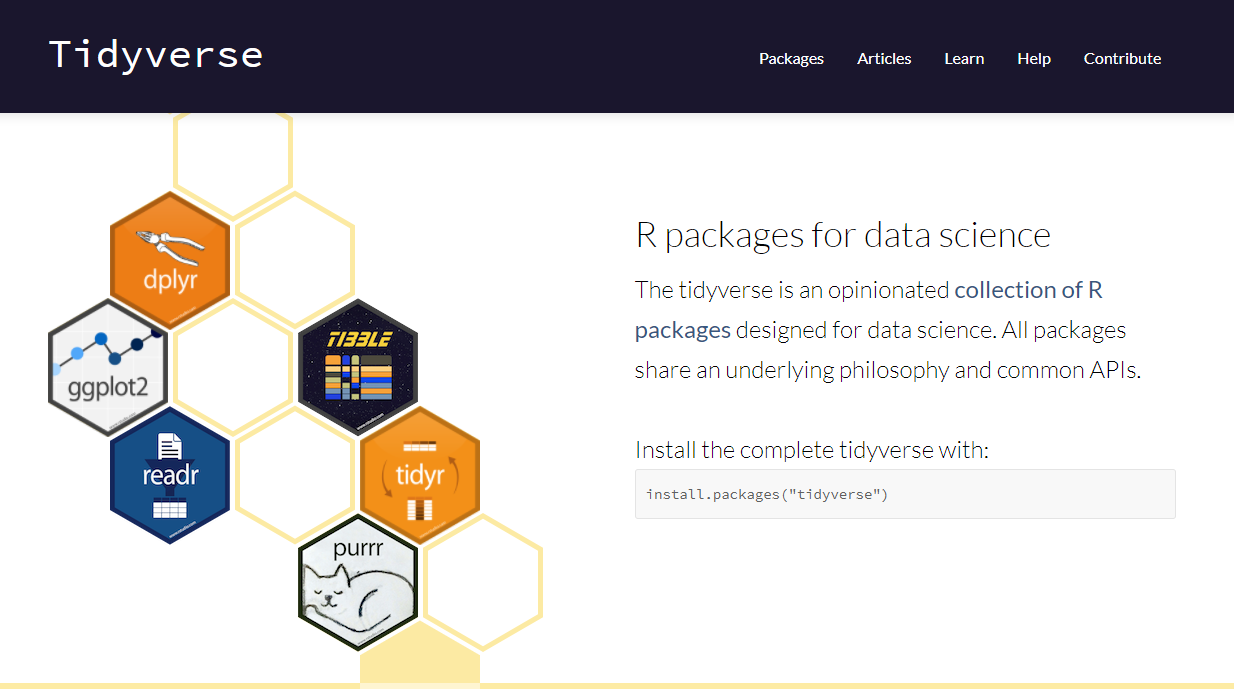
\includegraphics[width=0.55\linewidth]{imgs/2017/tidyverse} \end{center}
\end{frame}

\begin{frame}{SQL}
\protect\hypertarget{sql}{}
\begin{itemize}
\tightlist
\item
  It was invented by Edgar Codd
\item
  It first appeared in 1974, which is 46 years ago.
\end{itemize}

\begin{center}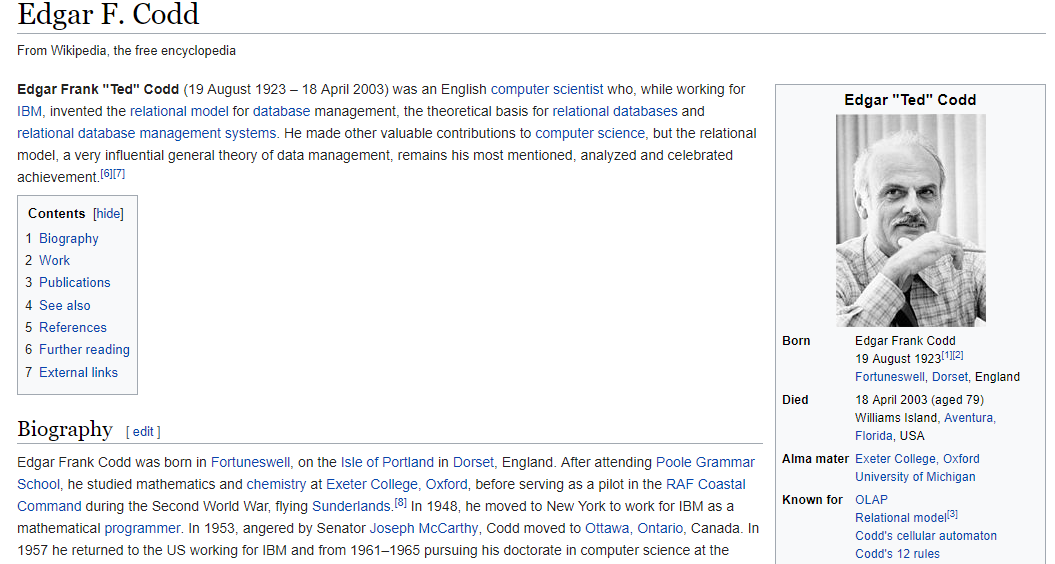
\includegraphics[width=0.6\linewidth]{imgs/2017/edgar-codd} \end{center}
\end{frame}

\begin{frame}{CRUD: Create \textbar{} Read \textbar{} Update \textbar{}
Delete}
\protect\hypertarget{crud-create-read-update-delete}{}
Data engineering was born around 70s with SQL.

\begin{center}
\includegraphics[width=0.45\linewidth]{imgs/2017/CRUD} \end{center}
\end{frame}

\begin{frame}[fragile]{SQL does CRUD}
\protect\hypertarget{sql-does-crud}{}
\begin{verbatim}
# Select everything from Shops.
SELECT * FROM Shops;

# Select with a filter
SELECT * FROM Shops WHERE size = "Big";

# Select with a filter and order
SELECT * FROM Shops WHERE size = "Big" ORDER BY Name;

# Select with a filter, order, group and summary function `sum`
SELECT Region, sum(Sales) FROM Shops WHERE size = "Medium" GROUP BY Region;

# Insert a new record to Shops.
INSERT into Shops (Name, Region, Sales) VALUES ("Costco", "North", 123456, ...);

# Update a field
UPDATE Shops SET Sales = Sales + 1000 WHERE Name = "Costco";

# Delete from Shops with a filter
DELETE from Shops WHERE Sales < 1000
\end{verbatim}
\end{frame}

\begin{frame}[fragile]{Data frame does CRUD}
\protect\hypertarget{data-frame-does-crud}{}
\begin{Shaded}
\begin{Highlighting}[]
\NormalTok{df \textless{}{-}}\StringTok{ }\KeywordTok{data.frame}\NormalTok{(}\DataTypeTok{a =} \DecValTok{1}\OperatorTok{:}\DecValTok{10}\NormalTok{, }\DataTypeTok{b =} \DecValTok{10}\OperatorTok{:}\DecValTok{1}\NormalTok{)}
\CommentTok{\# Select (aka Filter)}
\NormalTok{df[}\KeywordTok{which}\NormalTok{(df}\OperatorTok{$}\NormalTok{a }\OperatorTok{==}\StringTok{ }\DecValTok{3} \OperatorTok{|}\StringTok{ }\NormalTok{df}\OperatorTok{$}\NormalTok{b }\OperatorTok{==}\StringTok{ }\DecValTok{3}\NormalTok{), , drop =}\StringTok{ }\NormalTok{T] }
\NormalTok{df[}\KeywordTok{match}\NormalTok{(}\DecValTok{3}\NormalTok{, df}\OperatorTok{$}\NormalTok{a), , drop =}\StringTok{ }\NormalTok{T]}
\NormalTok{df[, }\KeywordTok{match}\NormalTok{(}\StringTok{"b"}\NormalTok{, }\KeywordTok{colnames}\NormalTok{(df)), drop =}\StringTok{ }\NormalTok{T] }

\CommentTok{\# Insert}
\KeywordTok{rbind}\NormalTok{(df, df)}

\CommentTok{\# Delete}
\NormalTok{df[}\OperatorTok{{-}}\NormalTok{(}\KeywordTok{which}\NormalTok{(df}\OperatorTok{$}\NormalTok{a }\OperatorTok{==}\StringTok{ }\DecValTok{3} \OperatorTok{|}\StringTok{ }\NormalTok{df}\OperatorTok{$}\NormalTok{b }\OperatorTok{==}\StringTok{ }\DecValTok{3}\NormalTok{)), , drop =}\StringTok{ }\NormalTok{T]}

\CommentTok{\# Update}
\NormalTok{df[}\KeywordTok{which}\NormalTok{(df}\OperatorTok{$}\NormalTok{a }\OperatorTok{==}\StringTok{ }\DecValTok{3} \OperatorTok{|}\StringTok{ }\NormalTok{df}\OperatorTok{$}\NormalTok{b }\OperatorTok{==}\StringTok{ }\DecValTok{3}\NormalTok{), }\DecValTok{2}\NormalTok{] \textless{}{-}}\StringTok{ }\DecValTok{3}
\end{Highlighting}
\end{Shaded}
\end{frame}

\begin{frame}[fragile]{dplyr}
\protect\hypertarget{dplyr}{}
dplyr package from tidyverse is a high-performance package to manipulate
data in data frame.

\begin{Shaded}
\begin{Highlighting}[]
\CommentTok{\# tidyverse is a bundle of packages.}
\CommentTok{\# I usually load them all with library(tidyverse, instead of library(dplyr) individually.}
\KeywordTok{library}\NormalTok{(tidyverse)}
\CommentTok{\# {-}{-} Attaching packages {-}{-}{-}{-}{-}{-}{-}{-}{-}{-}{-}{-}{-}{-}{-}{-}{-}{-}{-}{-}{-}{-}{-}{-}{-}{-}{-}{-}{-}{-}{-}{-}{-}{-}{-}{-}{-}{-}{-} tidyverse 1.2.1 {-}{-}}
\CommentTok{\# v ggplot2 3.2.1     v purrr   0.3.2}
\CommentTok{\# v tibble  2.1.3     v dplyr   0.8.3}
\CommentTok{\# v tidyr   0.8.3     v stringr 1.4.0}
\CommentTok{\# v readr   1.3.1     v forcats 0.4.0}
\CommentTok{\# {-}{-} Conflicts {-}{-}{-}{-}{-}{-}{-}{-}{-}{-}{-}{-}{-}{-}{-}{-}{-}{-}{-}{-}{-}{-}{-}{-}{-}{-}{-}{-}{-}{-}{-}{-}{-}{-}{-}{-}{-}{-}{-}{-}{-}{-} tidyverse\_conflicts() {-}{-}}
\CommentTok{\# x dplyr::filter() masks stats::filter()}
\CommentTok{\# x dplyr::lag()    masks stats::lag()}
\end{Highlighting}
\end{Shaded}

Use dplyr::lag and dplyr::filter when it doesn't work.
\end{frame}

\begin{frame}[fragile]{How dplyr works}
\protect\hypertarget{how-dplyr-works}{}
\texttt{dplyr} provides functions in ``verbs'', which is functions that
does one thing only. We will learn to use the following.

\begin{itemize}
\tightlist
\item
  Key

  \begin{itemize}
  \tightlist
  \item
    select: return a subset of the columns of a data frame
  \item
    filter: extract a subset of rows based on logical conditions
  \item
    arrange: reorder rows
  \item
    rename: rename variables
  \item
    mutate: add new variables/columns or transform existing variables
  \end{itemize}
\item
  Group

  \begin{itemize}
  \tightlist
  \item
    group\_by / rowwise / ungroup: stratify the data
  \item
    summarise / summarize: generate summary statistics of different
    variables in the data frame, possibly within strata
  \item
    do: process data within the strata
  \end{itemize}
\item
  Combine

  \begin{itemize}
  \tightlist
  \item
    left\_join / right\_join / anti\_join / full\_join
  \item
    bind\_rows / bind\_cols
  \end{itemize}
\item
  Helpers

  \begin{itemize}
  \tightlist
  \item
    \%\textgreater\%: the ``pipe'' operator is used to connect multiple
    verb actions together into a pipeline
  \item
    ifelse / case\_when
  \item
    lag/distinct
  \item
    n
  \end{itemize}
\end{itemize}
\end{frame}

\begin{frame}[fragile]{Sample dataset}
\protect\hypertarget{sample-dataset}{}
\begin{verbatim}
A data-driven approach to predict the success of telemarketing
Author: Sérgio Moroa; Paulo Cortezb; Paulo Ritaa
<http://dx.doi.org/10.1016/j.dss.2014.03.001>
\end{verbatim}

I chose this data set of a Portuguese retail bank clients profile.

\begin{itemize}
\tightlist
\item
  Real data collected from a Portuguese retailbank, from May 2008 to
  June 2013, in a total of 52,944 phone contacts.
\end{itemize}

\begin{center}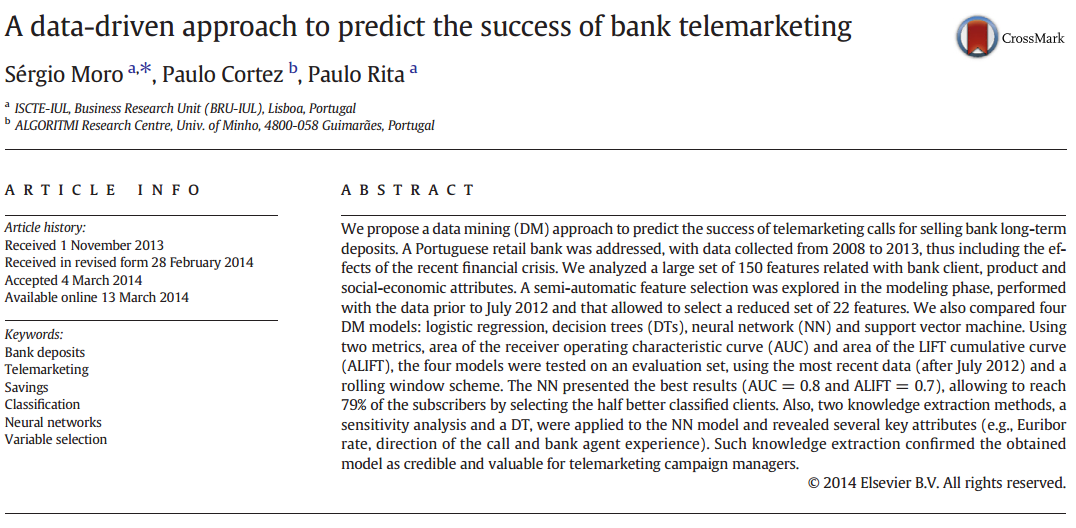
\includegraphics[width=0.45\linewidth]{imgs/2017/sample-bank-data} \end{center}
\end{frame}

\begin{frame}{Sample dataset columns (also called variable, field or
feature)}
\protect\hypertarget{sample-dataset-columns-also-called-variable-field-or-feature}{}
\begin{itemize}
\item
  Personal profile
\item
  1 - age (numeric)
\item
  2 - job : type of job (categorical:
  ``admin.'',``unknown'',``unemployed'',``management'',``housemaid'',``entrepreneur'',``student'',
  ``blue-collar'',``self-employed'',``retired'',``technician'',``services'')
\item
  3 - marital : marital status (categorical:
  ``married'',``divorced'',``single''; note: ``divorced'' means divorced
  or widowed)
\item
  4 - education (categorical:
  ``unknown'',``secondary'',``primary'',``tertiary'')
\item
  5 - default: has credit in default? (binary: ``yes'',``no'')
\item
  6 - balance: average yearly balance, in euros (numeric)
\item
  7 - housing: has housing loan? (binary: ``yes'',``no'')
\item
  8 - loan: has personal loan? (binary: ``yes'',``no'')
\item
  Related with the last contact of the current campaign:
\item
  9 - contact: contact communication type (categorical:
  ``unknown'',``telephone'',``cellular'')
\item
  10 - day: last contact day of the month (numeric)
\item
  11 - month: last contact month of year (categorical: ``jan'', ``feb'',
  ``mar'', \ldots, ``nov'', ``dec'')
\item
  12 - duration: last contact duration, in seconds (numeric)
\item
  Other attributes:
\item
  13 - campaign: number of contacts performed during this campaign and
  for this client (numeric, includes last contact)
\item
  14 - pdays: number of days that passed by after the client was last
  contacted from a previous campaign (numeric, -1 means client was not
  previously contacted)
\item
  15 - previous: number of contacts performed before this campaign and
  for this client (numeric)
\item
  16 - poutcome: outcome of the previous marketing campaign
  (categorical: ``unknown'',``other'',``failure'',``success'')
\item
  Output variable (desired target):
\item
  17 - y - has the client subscribed a term deposit? (binary:
  ``yes'',``no'')
\end{itemize}
\end{frame}

\begin{frame}[fragile]{Read data}
\protect\hypertarget{read-data}{}
Use RStudio's File -\textgreater{} Import Dataset, you may choose either
``From Text (base)'' or ``From Text (readr)''. Either way loads the
data.

\texttt{base} comes with R. \texttt{readr} is a package from tidyverse
that provides more options and functionality. Copy the generated code to
your script file.

I place it at \url{https://goo.gl/PBQnBt} (for direct use),
\url{https://goo.gl/fFQAAm} (for Download).

You may download it and save it to local.

\begin{Shaded}
\begin{Highlighting}[]
\CommentTok{\# Use base}
\NormalTok{bank \textless{}{-}}\StringTok{ }\KeywordTok{read.csv}\NormalTok{(}\StringTok{"example/data{-}bank/bank.csv"}\NormalTok{, }\DataTypeTok{sep=}\StringTok{";"}\NormalTok{) }\CommentTok{\# or,}
\NormalTok{bank \textless{}{-}}\StringTok{ }\KeywordTok{read.csv}\NormalTok{(}\StringTok{"https://goo.gl/PBQnBt"}\NormalTok{, }\DataTypeTok{sep =} \StringTok{";"}\NormalTok{)}

\CommentTok{\# use readr}
\KeywordTok{library}\NormalTok{(readr)}
\NormalTok{bank \textless{}{-}}\StringTok{ }\KeywordTok{read\_delim}\NormalTok{(}\StringTok{"example/data{-}bank/bank.csv"}\NormalTok{, }
                    \StringTok{";"}\NormalTok{, }\DataTypeTok{escape\_double =} \OtherTok{FALSE}\NormalTok{, }\DataTypeTok{trim\_ws =} \OtherTok{TRUE}\NormalTok{)}
\CommentTok{\#\# Parsed with column specification:}
\CommentTok{\#\# cols(}
\CommentTok{\#\#   age = col\_double(),}
\CommentTok{\#\#   job = col\_character(),}
\CommentTok{\#\#   marital = col\_character(),}
\CommentTok{\#\#   education = col\_character(),}
\CommentTok{\#\#   default = col\_character(),}
\CommentTok{\#\#   balance = col\_double(),}
\CommentTok{\#\#   housing = col\_character(),}
\CommentTok{\#\#   loan = col\_character(),}
\CommentTok{\#\#   contact = col\_character(),}
\CommentTok{\#\#   day = col\_double(),}
\CommentTok{\#\#   month = col\_character(),}
\CommentTok{\#\#   duration = col\_double(),}
\CommentTok{\#\#   campaign = col\_double(),}
\CommentTok{\#\#   pdays = col\_double(),}
\CommentTok{\#\#   previous = col\_double(),}
\CommentTok{\#\#   poutcome = col\_character(),}
\CommentTok{\#\#   y = col\_character()}
\CommentTok{\#\# )}
\end{Highlighting}
\end{Shaded}

\begin{Shaded}
\begin{Highlighting}[]
\KeywordTok{View}\NormalTok{(bank)}
\end{Highlighting}
\end{Shaded}
\end{frame}

\begin{frame}[fragile]{\texttt{select}}
\protect\hypertarget{select}{}
\texttt{select(df,\ ...)}, \ldots{} can be

\begin{itemize}
\tightlist
\item
  variable name
\item
  numeric to indicate nth column (\texttt{-} means exclude)
\item
  a range
\item
  a function
\end{itemize}
\end{frame}

\begin{frame}[fragile]{\texttt{select} - Examples}
\protect\hypertarget{select---examples}{}
\begin{Shaded}
\begin{Highlighting}[]
\NormalTok{subset \textless{}{-}}\StringTok{ }\KeywordTok{select}\NormalTok{(bank, marital)}
\NormalTok{subset \textless{}{-}}\StringTok{ }\KeywordTok{select}\NormalTok{(bank, }\DecValTok{1}\NormalTok{)}
\NormalTok{subset \textless{}{-}}\StringTok{ }\KeywordTok{select}\NormalTok{(bank, }\DecValTok{{-}1}\NormalTok{)}
\NormalTok{subset \textless{}{-}}\StringTok{ }\KeywordTok{select}\NormalTok{(bank, }\OperatorTok{{-}}\NormalTok{job)}
\NormalTok{subset \textless{}{-}}\StringTok{ }\KeywordTok{select}\NormalTok{(bank, }\OperatorTok{{-}}\NormalTok{(job}\OperatorTok{:}\NormalTok{education))}
\NormalTok{subset \textless{}{-}}\StringTok{ }\KeywordTok{select}\NormalTok{(bank, }\KeywordTok{starts\_with}\NormalTok{(}\StringTok{"p"}\NormalTok{))}
\NormalTok{subset \textless{}{-}}\StringTok{ }\KeywordTok{select}\NormalTok{(bank, }\KeywordTok{ends\_with}\NormalTok{(}\StringTok{"p"}\NormalTok{))}
\NormalTok{subset \textless{}{-}}\StringTok{ }\KeywordTok{select}\NormalTok{(bank, }\KeywordTok{contains}\NormalTok{(}\StringTok{"p"}\NormalTok{))}
\end{Highlighting}
\end{Shaded}
\end{frame}

\begin{frame}[fragile]{\texttt{select} as a re-arrangement of columns.}
\protect\hypertarget{select-as-a-re-arrangement-of-columns.}{}
\begin{Shaded}
\begin{Highlighting}[]
\NormalTok{job\_first \textless{}{-}}\StringTok{ }\KeywordTok{select}\NormalTok{(bank, job, }\KeywordTok{everything}\NormalTok{())}
\end{Highlighting}
\end{Shaded}
\end{frame}

\begin{frame}[fragile]{\texttt{filter}}
\protect\hypertarget{filter}{}
\begin{Shaded}
\begin{Highlighting}[]
\KeywordTok{colnames}\NormalTok{(bank)}
\CommentTok{\#\#  [1] "age"       "job"       "marital"   "education" "default"   "balance"  }
\CommentTok{\#\#  [7] "housing"   "loan"      "contact"   "day"       "month"     "duration" }
\CommentTok{\#\# [13] "campaign"  "pdays"     "previous"  "poutcome"  "y"}

\NormalTok{young \textless{}{-}}\StringTok{ }\NormalTok{dplyr}\OperatorTok{::}\KeywordTok{filter}\NormalTok{(bank, age }\OperatorTok{\textless{}}\StringTok{ }\DecValTok{40}\NormalTok{)}
\NormalTok{another\_young \textless{}{-}}\StringTok{ }\NormalTok{dplyr}\OperatorTok{::}\KeywordTok{filter}\NormalTok{(bank, age }\OperatorTok{\textless{}}\StringTok{ }\DecValTok{20} \OperatorTok{\&}\StringTok{ }\NormalTok{marital }\OperatorTok{==}\StringTok{ "married"}\NormalTok{)}
\NormalTok{just\_young \textless{}{-}}\StringTok{ }\NormalTok{dplyr}\OperatorTok{::}\KeywordTok{filter}\NormalTok{(bank, age }\OperatorTok{\textless{}}\StringTok{ }\DecValTok{20} \OperatorTok{\&}\StringTok{ }\NormalTok{marital }\OperatorTok{==}\StringTok{ "single"}\NormalTok{)}

\NormalTok{young2 \textless{}{-}}\StringTok{ }\NormalTok{dplyr}\OperatorTok{::}\KeywordTok{filter}\NormalTok{(bank, age }\OperatorTok{\textgreater{}=}\StringTok{ }\DecValTok{20} \OperatorTok{\&}\StringTok{ }\NormalTok{age }\OperatorTok{\textless{}}\StringTok{ }\DecValTok{30}\NormalTok{)}
\NormalTok{another\_young2 \textless{}{-}}\StringTok{ }\NormalTok{dplyr}\OperatorTok{::}\KeywordTok{filter}\NormalTok{(bank, age }\OperatorTok{\textgreater{}=}\StringTok{ }\DecValTok{20} \OperatorTok{\&}\StringTok{ }\NormalTok{age }\OperatorTok{\textless{}}\StringTok{ }\DecValTok{30} \OperatorTok{\&}\StringTok{ }\NormalTok{marital }\OperatorTok{==}\StringTok{ "married"}\NormalTok{)}
\NormalTok{just\_young2 \textless{}{-}}\StringTok{ }\NormalTok{dplyr}\OperatorTok{::}\KeywordTok{filter}\NormalTok{(bank, age }\OperatorTok{\textgreater{}=}\StringTok{ }\DecValTok{20} \OperatorTok{\&}\StringTok{ }\NormalTok{age }\OperatorTok{\textless{}}\StringTok{ }\DecValTok{30} \OperatorTok{\&}\StringTok{ }\NormalTok{marital }\OperatorTok{==}\StringTok{ "single"}\NormalTok{)}
\end{Highlighting}
\end{Shaded}
\end{frame}

\begin{frame}{\texttt{filter} - logic operators}
\protect\hypertarget{filter---logic-operators}{}
\begin{center}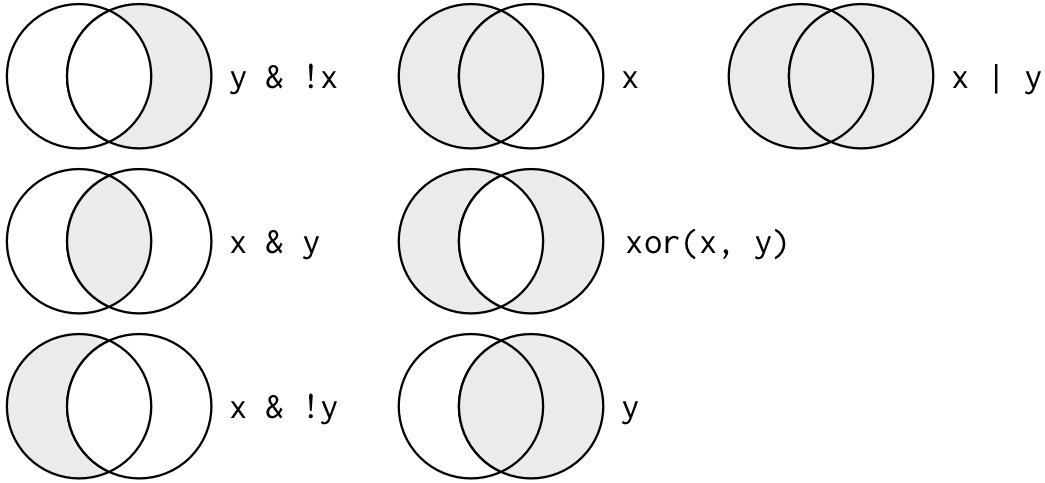
\includegraphics[width=0.75\linewidth]{imgs/2017/transform-logical} \end{center}
\end{frame}

\begin{frame}[fragile]{\texttt{filter} - string operations}
\protect\hypertarget{filter---string-operations}{}
\begin{Shaded}
\begin{Highlighting}[]
\CommentTok{\# \%in\% to match multiple}
\NormalTok{second\_upper \textless{}{-}}\StringTok{ }\NormalTok{dplyr}\OperatorTok{::}\KeywordTok{filter}\NormalTok{(bank, education }\OperatorTok{\%in\%}\StringTok{ }\KeywordTok{c}\NormalTok{(}\StringTok{"tertiary"}\NormalTok{, }\StringTok{"secondary"}\NormalTok{))}

\CommentTok{\# filter out NA value.}
\NormalTok{no\_na \textless{}{-}}\StringTok{ }\NormalTok{dplyr}\OperatorTok{::}\KeywordTok{filter}\NormalTok{(bank, }\OperatorTok{!}\KeywordTok{is.na}\NormalTok{(balance) }\OperatorTok{\&}\StringTok{ }\NormalTok{balance }\OperatorTok{\textgreater{}}\StringTok{ }\DecValTok{0}\NormalTok{)}
\end{Highlighting}
\end{Shaded}
\end{frame}

\begin{frame}{Exercise}
\protect\hypertarget{exercise}{}
\begin{itemize}
\tightlist
\item
  How many bank client have a loan while doesn't have a housing?
\item
  How many bank client have a job between 20 to 40?
\end{itemize}
\end{frame}

\begin{frame}[fragile]{\texttt{rename}}
\protect\hypertarget{rename}{}
\begin{Shaded}
\begin{Highlighting}[]
\CommentTok{\# rename(new name = old)}
\CommentTok{\# Use tick to quote special strings.}
\NormalTok{df \textless{}{-}}\StringTok{ }\KeywordTok{rename}\NormalTok{(bank, }\DataTypeTok{young\_age =}\NormalTok{ age) }
\NormalTok{df \textless{}{-}}\StringTok{ }\KeywordTok{rename}\NormalTok{(bank, }\StringTok{\textasciigrave{}}\DataTypeTok{Age in Bank}\StringTok{\textasciigrave{}}\NormalTok{ =}\StringTok{ }\NormalTok{age)}
\end{Highlighting}
\end{Shaded}
\end{frame}

\begin{frame}[fragile]{\texttt{arrange}}
\protect\hypertarget{arrange}{}
\begin{Shaded}
\begin{Highlighting}[]
\CommentTok{\# arrange is sort}
\KeywordTok{arrange}\NormalTok{(bank, job)}
\KeywordTok{arrange}\NormalTok{(bank, default, job)}

\CommentTok{\# descending for day}
\KeywordTok{arrange}\NormalTok{(bank, }\KeywordTok{desc}\NormalTok{(day))}
\KeywordTok{arrange}\NormalTok{(bank, }\KeywordTok{desc}\NormalTok{(}\KeywordTok{as.Date}\NormalTok{(day, }\DataTypeTok{format=}\StringTok{"\%d"}\NormalTok{, }\DataTypeTok{origin =} \KeywordTok{Sys.Date}\NormalTok{())))}
\end{Highlighting}
\end{Shaded}

NB: Missing values are always sorted at the end.
\end{frame}

\begin{frame}[fragile]{Exercise}
\protect\hypertarget{exercise-1}{}
\begin{itemize}
\tightlist
\item
  How could you use arrange() to sort all missing values to the start?
  (Hint: use \texttt{is.na()}).
\end{itemize}

\begin{Shaded}
\begin{Highlighting}[]
\KeywordTok{arrange}\NormalTok{(bank, }\OperatorTok{!}\KeywordTok{is.na}\NormalTok{(a), a)}
\end{Highlighting}
\end{Shaded}

\begin{itemize}
\tightlist
\item
  Find the longest duration?
\item
  Find the eldest?
\end{itemize}
\end{frame}

\begin{frame}[fragile]{\texttt{mutate}}
\protect\hypertarget{mutate}{}
\begin{Shaded}
\begin{Highlighting}[]
\CommentTok{\# Replace existing}
\CommentTok{\# ifelse is to check condition.}
\NormalTok{df1 \textless{}{-}}\StringTok{ }\KeywordTok{mutate}\NormalTok{(bank, }\DataTypeTok{y =} \KeywordTok{ifelse}\NormalTok{(y }\OperatorTok{==}\StringTok{ "yes"}\NormalTok{, T, F))}

\CommentTok{\# Add a new column.}
\NormalTok{df2 \textless{}{-}}\StringTok{ }\KeywordTok{mutate}\NormalTok{(bank, }\DataTypeTok{duration\_diff =}\NormalTok{ duration }\OperatorTok{{-}}\StringTok{ }\KeywordTok{mean}\NormalTok{(duration, }\DataTypeTok{na.rm =} \OtherTok{TRUE}\NormalTok{))}

\CommentTok{\# case\_when is a function to deal multiple choices.}
\NormalTok{df2\_age\_group \textless{}{-}}\StringTok{ }\KeywordTok{mutate}\NormalTok{(bank, }\DataTypeTok{age\_group =} \KeywordTok{case\_when}\NormalTok{(}
\NormalTok{  age }\OperatorTok{\textless{}}\StringTok{ }\DecValTok{20} \OperatorTok{\textasciitilde{}}\StringTok{ "youth"}\NormalTok{,}
\NormalTok{  age }\OperatorTok{\textless{}}\StringTok{ }\DecValTok{40} \OperatorTok{\textasciitilde{}}\StringTok{ "middle{-}age"}\NormalTok{,}
\NormalTok{  age }\OperatorTok{\textless{}}\StringTok{ }\DecValTok{50} \OperatorTok{\textasciitilde{}}\StringTok{ "senior"}\NormalTok{,}
  \OtherTok{TRUE} \OperatorTok{\textasciitilde{}}\StringTok{ "happy"}
\NormalTok{))}

\NormalTok{df2\_age\_group\_res \textless{}{-}}
\StringTok{  }\KeywordTok{group\_by}\NormalTok{(df2\_age\_group, age\_group) }\OperatorTok{\%\textgreater{}\%}
\StringTok{  }\KeywordTok{summarise}\NormalTok{(}\DataTypeTok{mean\_age =} \KeywordTok{mean}\NormalTok{(age)) }\OperatorTok{\%\textgreater{}\%}
\StringTok{  }\KeywordTok{transmute}\NormalTok{(}\DataTypeTok{mean\_age\_diff =}\NormalTok{ mean\_age }\OperatorTok{{-}}\StringTok{ }\KeywordTok{lag}\NormalTok{(mean\_age))}
\CommentTok{\#\# \textasciigrave{}summarise()\textasciigrave{} ungrouping output (override with \textasciigrave{}.groups\textasciigrave{} argument)}
\end{Highlighting}
\end{Shaded}
\end{frame}

\begin{frame}[fragile]{\texttt{mutate} 2}
\protect\hypertarget{mutate-2}{}
\begin{Shaded}
\begin{Highlighting}[]
\NormalTok{firstup \textless{}{-}}\StringTok{ }\ControlFlowTok{function}\NormalTok{(x) \{}
  \KeywordTok{substr}\NormalTok{(x, }\DecValTok{1}\NormalTok{, }\DecValTok{1}\NormalTok{) \textless{}{-}}\StringTok{ }\KeywordTok{toupper}\NormalTok{(}\KeywordTok{substr}\NormalTok{(x, }\DecValTok{1}\NormalTok{, }\DecValTok{1}\NormalTok{))}
\NormalTok{  x}
\NormalTok{\}}

\CommentTok{\# month.abb is a built{-}in array of month names.}
\NormalTok{df3 \textless{}{-}}\StringTok{ }\KeywordTok{mutate}\NormalTok{(bank, }\DataTypeTok{month\_name =} \KeywordTok{factor}\NormalTok{(}\KeywordTok{firstup}\NormalTok{(}\KeywordTok{as.character}\NormalTok{(month)), }\DataTypeTok{levels =}\NormalTok{ month.abb))}

\CommentTok{\# transmute would remove all other columns after mutation, only keeping the new variable.}
\NormalTok{df5 \textless{}{-}}\StringTok{ }\KeywordTok{transmute}\NormalTok{(bank, }
                  \DataTypeTok{duration\_trend =}\NormalTok{ duration }\OperatorTok{{-}}\StringTok{ }\KeywordTok{mean}\NormalTok{(duration, }\DataTypeTok{na.rm =} \OtherTok{TRUE}\NormalTok{),}
                  \DataTypeTok{balance\_trend =}\NormalTok{ balance }\OperatorTok{{-}}\StringTok{ }\KeywordTok{mean}\NormalTok{(balance, }\DataTypeTok{na.rm =} \OtherTok{TRUE}\NormalTok{))}
\end{Highlighting}
\end{Shaded}
\end{frame}

\begin{frame}[fragile]{What you can do with \texttt{mutate}}
\protect\hypertarget{what-you-can-do-with-mutate}{}
\begin{itemize}
\tightlist
\item
  +, -, *, /: ordinary arithmetic operator
\item
  \%/\% (integer division) and \%\% (remainder), where x == y * (x \%/\%
  y) + (x \%\% y)
\item
  x / sum(x): compute the proportion of all things
\item
  y - mean(y): computes the difference from the mean.
\item
  log2(), log(), log10():
\item
  lead(), lag(): compute running differences (e.g.~x - lag(x)) or find
  when values change (x != lag(x)
\item
  rolling sum, prod, min, max: cumsum(), cumprod(), cummin(), cummax();
  and dplyr provides cummean()
\item
  row\_number()/min\_rank()/ntile(,n)
\end{itemize}

\begin{Shaded}
\begin{Highlighting}[]
\NormalTok{y \textless{}{-}}\StringTok{ }\KeywordTok{c}\NormalTok{(}\DecValTok{1}\NormalTok{, }\DecValTok{2}\NormalTok{, }\DecValTok{2}\NormalTok{, }\OtherTok{NA}\NormalTok{, }\DecValTok{3}\NormalTok{, }\DecValTok{4}\NormalTok{)}
\KeywordTok{row\_number}\NormalTok{(y)}
\CommentTok{\#\# [1]  1  2  3 NA  4  5}
\KeywordTok{min\_rank}\NormalTok{(y)}
\CommentTok{\#\# [1]  1  2  2 NA  4  5}
\KeywordTok{ntile}\NormalTok{(y, }\DecValTok{2}\NormalTok{)}
\CommentTok{\#\# [1]  1  1  1 NA  2  2}
\end{Highlighting}
\end{Shaded}
\end{frame}

\begin{frame}{Summary}
\protect\hypertarget{summary}{}
\begin{itemize}
\tightlist
\item
  We learned the key ``verbs'' from dplyr. Let's pick up the rest next
  week.
\end{itemize}
\end{frame}

\begin{frame}[fragile]{Pipe: \%\textgreater\%}
\protect\hypertarget{pipe}{}
We may write such code.

\begin{Shaded}
\begin{Highlighting}[]
\NormalTok{df \textless{}{-}}\StringTok{ }\KeywordTok{select}\NormalTok{(df, x)}
\NormalTok{df \textless{}{-}}\StringTok{ }\KeywordTok{mutate}\NormalTok{(df, }\DataTypeTok{a =} \DecValTok{1}\NormalTok{)}
\NormalTok{df \textless{}{-}}\StringTok{ }\KeywordTok{rename}\NormalTok{(df, }\DataTypeTok{a =}\NormalTok{ b)}
\NormalTok{df \textless{}{-}}\StringTok{ }\KeywordTok{arrange}\NormalTok{(df, x)}

\CommentTok{\# This is effectively,}
\KeywordTok{arrange}\NormalTok{(}\KeywordTok{rename}\NormalTok{(}\KeywordTok{mutate}\NormalTok{(}\KeywordTok{select}\NormalTok{(df, x), }\DataTypeTok{a =} \DecValTok{1}\NormalTok{), }\DataTypeTok{a =}\NormalTok{ b), x)}

\KeywordTok{third}\NormalTok{(}\KeywordTok{second}\NormalTok{(}\KeywordTok{first}\NormalTok{(x)))}
\end{Highlighting}
\end{Shaded}

How about this?

\begin{Shaded}
\begin{Highlighting}[]
\NormalTok{df }\OperatorTok{\%\textgreater{}\%}\StringTok{ }\NormalTok{select }\OperatorTok{\%\textgreater{}\%}\StringTok{ }\NormalTok{mutate }\OperatorTok{\%\textgreater{}\%}\StringTok{ }\NormalTok{rename }\OperatorTok{\%\textgreater{}\%}\StringTok{ }\NormalTok{arrange}
\end{Highlighting}
\end{Shaded}
\end{frame}

\begin{frame}[fragile]{\%\textgreater\% Benefits}
\protect\hypertarget{benefits}{}
\texttt{\%\textgreater{}\%} operator allows you to transform the flow
from nesting to left-to-right fashion, i.e.

\begin{Shaded}
\begin{Highlighting}[]
\KeywordTok{first}\NormalTok{(x) }\OperatorTok{\%\textgreater{}\%}\StringTok{ }\KeywordTok{second}\NormalTok{() }\OperatorTok{\%\textgreater{}\%}\StringTok{ }\KeywordTok{third}\NormalTok{()}

\NormalTok{x }\OperatorTok{\%\textgreater{}\%}\StringTok{ }\KeywordTok{first}\NormalTok{() }\OperatorTok{\%\textgreater{}\%}\StringTok{ }\KeywordTok{second}\NormalTok{() }\OperatorTok{\%\textgreater{}\%}\StringTok{ }\KeywordTok{third}\NormalTok{() }\CommentTok{\# this could also do.}

\NormalTok{x }\OperatorTok{\%\textgreater{}\%}\StringTok{ }\KeywordTok{first}\NormalTok{(.) }\OperatorTok{\%\textgreater{}\%}\StringTok{ }\KeywordTok{second}\NormalTok{(.) }\OperatorTok{\%\textgreater{}\%}\StringTok{ }\KeywordTok{third}\NormalTok{(.) }\CommentTok{\# . represents the input}
\end{Highlighting}
\end{Shaded}

What's the output of below?

\begin{Shaded}
\begin{Highlighting}[]
\KeywordTok{c}\NormalTok{(}\DecValTok{1}\NormalTok{, }\DecValTok{3}\NormalTok{, }\DecValTok{7}\NormalTok{, }\DecValTok{9}\NormalTok{) }\OperatorTok{\%\textgreater{}\%}\StringTok{ }\NormalTok{\{}
  \KeywordTok{print}\NormalTok{(.)}
  \KeywordTok{mean}\NormalTok{(.)}
\NormalTok{\} }\OperatorTok{\%\textgreater{}\%}\StringTok{ }\NormalTok{\{ . }\OperatorTok{*}\StringTok{ }\DecValTok{3}\NormalTok{ \} }\OperatorTok{\%\textgreater{}\%}\StringTok{ }\NormalTok{\{}
  \KeywordTok{print}\NormalTok{(.)}
  \KeywordTok{sample}\NormalTok{(}\KeywordTok{round}\NormalTok{(., }\DecValTok{0}\NormalTok{))}
\NormalTok{\}}
\CommentTok{\#\# [1] 1 3 7 9}
\CommentTok{\#\# [1] 15}
\CommentTok{\#\#  [1]  9 14  5  3  4  8 10 15  1 12  2  7 11  6 13}
\end{Highlighting}
\end{Shaded}
\end{frame}

\begin{frame}[fragile]{Work with Pipe}
\protect\hypertarget{work-with-pipe}{}
\%\textgreater\% \ldots{} \%\textgreater\%

\begin{Shaded}
\begin{Highlighting}[]
\CommentTok{\# Feed the data for multiple processing}
\NormalTok{\{}
\NormalTok{  v \textless{}{-}}\StringTok{ }\NormalTok{.}
\NormalTok{  cn \textless{}{-}}\StringTok{ }\KeywordTok{colnames}\NormalTok{(v)}

\NormalTok{  v \textless{}{-}}\StringTok{ }\KeywordTok{select}\NormalTok{(v, u, z)}
  \KeywordTok{colnames}\NormalTok{(v) \textless{}{-}}\StringTok{ }\NormalTok{cn[}\DecValTok{1}\OperatorTok{:}\DecValTok{3}\NormalTok{]}
\NormalTok{  v}
\NormalTok{\} }

\CommentTok{\# How to return multiple value}

\OperatorTok{\%\textgreater{}\%}\StringTok{ }\NormalTok{\{}
  \KeywordTok{assign}\NormalTok{(}\StringTok{"new\_data"}\NormalTok{, }\KeywordTok{filter}\NormalTok{(., group }\OperatorTok{==}\StringTok{ "1"}\NormalTok{), }\DataTypeTok{envir =} \KeywordTok{parent.env}\NormalTok{(}\KeywordTok{environment}\NormalTok{()) )}
  \KeywordTok{filter}\NormalTok{(., group }\OperatorTok{==}\StringTok{ "2"}\NormalTok{)}
\NormalTok{\} }\OperatorTok{\%\textgreater{}\%}\StringTok{ }\NormalTok{\{}
  \KeywordTok{select}\NormalTok{(., z }\OperatorTok{\textless{}}\StringTok{ }\FloatTok{0.4}\NormalTok{) }\CommentTok{\# on group 2}
  \KeywordTok{select}\NormalTok{(new\_data, z }\OperatorTok{\textgreater{}}\StringTok{ }\FloatTok{0.4}\NormalTok{) }\CommentTok{\# on group 1}
\NormalTok{\}}

\CommentTok{\# or, we use list}
\OperatorTok{\%\textgreater{}\%}\StringTok{ }\NormalTok{\{}
\NormalTok{  a \textless{}{-}}\StringTok{ }\KeywordTok{filter}\NormalTok{(., group }\OperatorTok{==}\StringTok{ "1"}\NormalTok{)}
\NormalTok{  b \textless{}{-}}\StringTok{ }\KeywordTok{filter}\NormalTok{(., group }\OperatorTok{==}\StringTok{ "2"}\NormalTok{)}
  \KeywordTok{list}\NormalTok{(a, b)}
\NormalTok{\}  }\OperatorTok{\%\textgreater{}\%}\StringTok{ }\NormalTok{\{}
\NormalTok{  v \textless{}{-}}\StringTok{ }\NormalTok{.}
\NormalTok{  v}\OperatorTok{$}\NormalTok{a}
\NormalTok{  v}\OperatorTok{$}\NormalTok{b}
\NormalTok{\}}
\end{Highlighting}
\end{Shaded}
\end{frame}

\begin{frame}[fragile]{Code pattern with Pipe}
\protect\hypertarget{code-pattern-with-pipe}{}
\begin{Shaded}
\begin{Highlighting}[]
\NormalTok{df }\OperatorTok{\%\textgreater{}\%}
\NormalTok{... }\OperatorTok{\%\textgreater{}\%}
\NormalTok{... }\OperatorTok{\%\textgreater{}\%}
\NormalTok{... }\OperatorTok{\%\textgreater{}\%}
\NormalTok{\{}
\NormalTok{  v \textless{}{-}}\StringTok{ }\NormalTok{.}
  \KeywordTok{ggplot}\NormalTok{(}\DataTypeTok{data =}\NormalTok{ v) }\OperatorTok{+}\StringTok{ }
\StringTok{    }\CommentTok{\# full data is used here}
\StringTok{    }\KeywordTok{geom\_line}\NormalTok{(}\DataTypeTok{data =}\NormalTok{ v) }\OperatorTok{+}
\StringTok{    }\CommentTok{\# partial data needs to be hightlighted.}
\StringTok{    }\KeywordTok{geom\_line}\NormalTok{(}\DataTypeTok{data =} \KeywordTok{filter}\NormalTok{(., some condition), }\DataTypeTok{color =} \StringTok{"red"}\NormalTok{)}
\NormalTok{\}}
\end{Highlighting}
\end{Shaded}
\end{frame}

\begin{frame}[fragile]{Use of Caution for Pipe (\%\textgreater\%)}
\protect\hypertarget{use-of-caution-for-pipe}{}
Pros:

\begin{itemize}
\tightlist
\item
  We don't need to keep intermediate result, sames memory and also
  variable names.
\end{itemize}

Cons:

\begin{itemize}
\item
  Difficult to debug, to find something in the middle of the chain.
\item
  Use \texttt{\{\ print(.);\ filter(.,\ ...)\ \}} to print intermediate
  resuls.
\item
  Separate the long pipes into shorter pipes, adding more intermediate
  variables.
\item
  Your pipes are longer than (say) ten steps. In that case, create
  intermediate objects with meaningful names. That will make debugging
  easier, because you can more easily check the intermediate results,
  and it makes it easier to understand your code, because the variable
  names can help communicate intent.
\item
  You have multiple inputs or outputs. If two or more objects being
  combined together, don't use the pipe.
\item
  Pipes are fundamentally linear and expressing complex relationships
  with them will typically yield confusing code.
\end{itemize}
\end{frame}

\begin{frame}[fragile]{Environment}
\protect\hypertarget{environment}{}
Environment is where your data resides. Use \texttt{local()} to isolate.

\begin{Shaded}
\begin{Highlighting}[]
\CommentTok{\# local stores the data wihtin the boundary of \{\}}
\NormalTok{x \textless{}{-}}\StringTok{ }\DecValTok{3}
\KeywordTok{local}\NormalTok{(\{}
  \KeywordTok{print}\NormalTok{(x)}
\NormalTok{  x \textless{}{-}}\StringTok{ }\DecValTok{1}
  \KeywordTok{print}\NormalTok{(x)}
\NormalTok{\})}
\CommentTok{\#\# [1] 3}
\CommentTok{\#\# [1] 1}
\KeywordTok{print}\NormalTok{(x)}
\CommentTok{\#\# [1] 3}
\end{Highlighting}
\end{Shaded}

\begin{Shaded}
\begin{Highlighting}[]
\CommentTok{\# local stores the nearest environment}
\NormalTok{x \textless{}{-}}\StringTok{ }\DecValTok{3}
\NormalTok{\{}
  \KeywordTok{print}\NormalTok{(x)}
\NormalTok{  x \textless{}{-}}\StringTok{ }\DecValTok{1}
  \KeywordTok{print}\NormalTok{(x)}
\NormalTok{\}}
\CommentTok{\#\# [1] 3}
\CommentTok{\#\# [1] 1}
\NormalTok{x}
\CommentTok{\#\# [1] 1}
\end{Highlighting}
\end{Shaded}

\begin{Shaded}
\begin{Highlighting}[]
\NormalTok{get\_sum \textless{}{-}}\StringTok{ }\ControlFlowTok{function}\NormalTok{(i) \{}
\NormalTok{  v \textless{}{-}}\StringTok{ }\DecValTok{0}
  \ControlFlowTok{for}\NormalTok{ (i }\ControlFlowTok{in} \DecValTok{1}\OperatorTok{:}\DecValTok{10}\NormalTok{) \{}
\NormalTok{    v \textless{}{-}}\StringTok{ }\NormalTok{v }\OperatorTok{+}\StringTok{ }\NormalTok{i}
\NormalTok{  \}}
\NormalTok{  v}
\NormalTok{\}}

\KeywordTok{get\_sum}\NormalTok{(}\DecValTok{10}\NormalTok{)}
\CommentTok{\#\# [1] 55}

\CommentTok{\# Error with line below: object \textquotesingle{}v\textquotesingle{} not found}
\CommentTok{\# v}
\end{Highlighting}
\end{Shaded}
\end{frame}

\begin{frame}[fragile]{Environment}
\protect\hypertarget{environment-1}{}
Use \texttt{assign()} to do space-jump.

\begin{Shaded}
\begin{Highlighting}[]
\CommentTok{\# assign data to global environment}
\NormalTok{x \textless{}{-}}\StringTok{ }\DecValTok{1}
\NormalTok{pass\_out\_global \textless{}{-}}\StringTok{ }\ControlFlowTok{function}\NormalTok{() \{}
  \KeywordTok{assign}\NormalTok{(}\StringTok{"x"}\NormalTok{, }\DecValTok{3}\NormalTok{, }\DataTypeTok{envir =}\NormalTok{ .GlobalEnv)  }
\NormalTok{\}}

\CommentTok{\# assign data to just one level up }
\NormalTok{pass\_out \textless{}{-}}\StringTok{ }\ControlFlowTok{function}\NormalTok{(env) \{}
  \KeywordTok{print}\NormalTok{(env)}
  \KeywordTok{assign}\NormalTok{(}\StringTok{"x"}\NormalTok{, }\DecValTok{2}\NormalTok{, }\DataTypeTok{envir =}\NormalTok{ env)}
\NormalTok{\}}
\end{Highlighting}
\end{Shaded}

\begin{Shaded}
\begin{Highlighting}[]
\NormalTok{x \textless{}{-}}\StringTok{ }\DecValTok{1}
\KeywordTok{pass\_out}\NormalTok{(}\KeywordTok{environment}\NormalTok{())}
\CommentTok{\#\# \textless{}environment: R\_GlobalEnv\textgreater{}}
\NormalTok{x}
\CommentTok{\#\# [1] 2}

\CommentTok{\# assign data to pass it out of function}
\NormalTok{extra\_layer \textless{}{-}}\StringTok{ }\ControlFlowTok{function}\NormalTok{(env) \{}
  \KeywordTok{pass\_out}\NormalTok{(env)}
\NormalTok{\}}

\NormalTok{x \textless{}{-}}\StringTok{ }\DecValTok{1}
\KeywordTok{extra\_layer}\NormalTok{(}\DataTypeTok{env =} \KeywordTok{environment}\NormalTok{())}
\CommentTok{\#\# \textless{}environment: R\_GlobalEnv\textgreater{}}
\NormalTok{x}
\CommentTok{\#\# [1] 2}

\NormalTok{extra\_layer\_g \textless{}{-}}\StringTok{ }\ControlFlowTok{function}\NormalTok{() \{}
  \KeywordTok{pass\_out\_global}\NormalTok{()}
\NormalTok{\}}

\NormalTok{x \textless{}{-}}\StringTok{ }\DecValTok{1}
\KeywordTok{extra\_layer\_g}\NormalTok{()}
\NormalTok{x}
\CommentTok{\#\# [1] 3}
\end{Highlighting}
\end{Shaded}
\end{frame}

\end{document}
